\chapter{Theoretical Background}
\label{chapter:background}
\epigraph{\textit{melody that will draw you into infinite darkness}}{Ocarina of Time}

Convolutional neural networks trained on large databases \cite{mnist2012,imagenet2009} have shaped machine learning research over the past couple of decades. Today they serve as canonical learning material in courses and are often used as initial \textit{vanilla} approaches for data exploration and classification tasks and before creating more bespoke machine learning pipelines. The widespread success of much models created an expectation in the research community that with sufficient data and computational power provided by one of the reigning consumer internet businesses, a data-driven black-box model can be created for any application ranging from quantum mechanics to economics. Convolutional architectures together with language models eventually inspired recurrent architectures and attention models where are the key ingredients in the creation of \textit{Alpha Fold} \cite{Jumper2021HighlyAlphaFold} that takes a substantial step towards solving the protein-folding problem. Biotechnology researchers are eager to apply these methods but face the following obstacles

In practice we can only observe a subset of the states $u$, for example by incorporating fluorescent proteins downstream of the coding sequences of the proteins that participate in the  mechanism. Incorporating any fluorescent proteins into the host genome contributes to cell burdon, at worst can disrupt the mechanism under study, and therefore incorporation sites much be chosen sparsely such that the bifurcation is still observable in the data.

\begin{itemize}
    \item \textbf{Insufficient data} due to strategic experimental designs 
    \item \textbf{Low extrapolation accuracy} for black box-models
\end{itemize}

In this section we will set the scene for chemical reaction systems and their
methods of analysis of steady state and network perspectives. Dynamical
methods makes use of field flow, linear stability and bifurcation analysis.

\section{Describing Phenotypes with Bifurcations}

\begin{equation}
	\frac{\partial u}{\partial t} = F(u,t)
	\label{eq:odes}
\end{equation}

Consider $N$ particles of $S$ species in a finite volume $\Omega$. These particles
can undergo $R$ possible reactions when they meet within the volume. Suppose the
timescales of equilibration with respect to volume and temperature are much faster
than that of species number equilibration. This means that non-reactive collisions
occur more frequently than collisions that trigger any of the $R$ reactions. This
is the essence of the \textit{well-mixed} approximation \cite{Gillespie1992}.

This suggests that at any time $t$ we may ignore spatial inhomogeneities and pin
down the state of the system by a vector of species populations $s(t)\in\mathbb{N}^S$.
All possible reactions in the mixture are encoded into a stoichiometric matrix
$\mathbf{\Gamma}\in\mathbb{Z}^{S\times R}$ whose columns $\mathbf{\Gamma}[r]\in\mathbb{Z}^{S}$
represent the population change vector for a given reaction $r$. Each reaction
has a propensity $\omega(r|s)\in[0,\infty)$ defined though transition
probabilities for an infinitesimal time interval given population $s$;
\begin{align}
	\omega(r|s)\mathrm{d}t := \mathbb{P}(s+\mathbf{\Gamma}[r],t+\mathrm{d}t|s,t)
	\label{eq:fundamentalpremise}
\end{align}
Suppose $\sigma[r]\mathrm{d}t$ gives the probability that the reaction $r$
will occur within the time interval $\mathrm{d}t$ independent of population
$s$. The constant $\sigma[r]$ could be in principle calculated from the
microscopic physics of the reaction. In quantum mechanics this would involve
calculating the wavefunction overlap or transition rates between initial and
final configurations.

The propensity is proportional this rate, up to combinatoric multiplicity
taking into account the species population $s$. A reaction $r$ chooses $g[i,r]$
particles for each reactant species $i$ from the $well-mixed$ solution containing
$s[i]$ particles. Thus the multiplicity is simply given by a binomial coefficient
per species. This results in a propensity that is polynomial in the components
$s[i]$, where the highest power term gives us the \textit{order} of the reaction.
\begin{align}
	\omega(r|s)=
	\sigma[r]
		\prod_{i=1}^S{s[i] \choose g[i,r]}
	\label{eq:propensity}
\end{align}
For reactions involving distinguishable particle species, all
components $ g[i,r]\in\{ 0,1\}$ and simplifies the combinatoric term to a
product of all reactant populations.
\begin{align}
	g[i,r]\in\{ 0,1\}\quad\forall i,r\quad\implies\quad
	\omega(r|s)=
	\sigma[r]
	\prod_{i=1}^S s[i]^{g[i,r]}
	\label{eq:simplifiedpropensity}
\end{align}
\subsection{Chemical Master Equation}
By applying the laws of probability and taking the $\mathrm{d}t\rightarrow 0$
one can derive a time-evolution equation
$\mathbb{P}(s,t)$ involving the definition \eqref{eq:fundamentalpremise} which
has become known as the Chemical Master Equation \cite{Gillespie1992,Gillespie2007}.
Note here the complexity lies within the non-linear state dependence in the propensity
$\omega(r|s)$. Were it not for this, we could solve this equation using
spectral methods.
\begin{align}
	\partial_t\mathbb{P}(s,t) &=
	\sum_{r=1}^R
	\omega(r|s-\mathbf{\Gamma}[r])\mathbb{P}(s-\mathbf{\Gamma}[r],t)-\omega(r|s)\mathbb{P}(s,t)
	\label{eq:cme}
\end{align}
Multiplying the Chemical Master Equation \eqref{eq:cme} by $s$ and summing over all $s$
obtains a system of differential equations for the first moment
$\left\langle s \right\rangle$ in terms of vectorised propensity
$\omega(s|\mathbf{\Gamma})\in[0,\infty)^R$ which couples to higher order moments,
unfolding an infinte heirarchy.
\begin{align}
	\partial_t
	\left\langle s \right\rangle &=
	\mathbf{\Gamma} \big\langle \omega(s|\mathbf{\Gamma}) \big\rangle
	\label{eq:momentheirarchy}
\end{align}
\subsection{Reaction Equation}
The mean field approximation factorises higher order moments, implying
$\big\langle f(s) \big\rangle=f(\langle s\rangle)$ for any nonlinear
function $f$. This is equivalent to neglecting fluctuations in the
$N,\Omega\rightarrow\infty$
thermodynamic limit, and it is here where the mass-action assumption
becomes manifest \cite{Gillespie2007}.

This closes the infinite heirarchy
\eqref{eq:momentheirarchy} yielding a nonlinear set of coupled ordinary
differential equations for a continuous vector field $\psi(t)\in[0,\infty)^S$.
These have come to be known as the Reaction Rate Equations, and are
typical for modelling processes in systems biology.
\begin{align}
	\partial_t
	\psi &=
	\mathbf{\Gamma}\omega(\psi|\mathbf{\Gamma})
	\label{eq:reaction}
\end{align}

\subsection{Bifurcation Analysis}
In the mean field approximation \eqref{eq:reaction} we may investigate the
steady state $\partial_t\psi=0$. This gives rise to a set of $S$ polynomial
equations in the components $\psi[s]\in[0,\infty)$ of steady state $\psi^*$
These define $S-1$ dimensional nullcline hypersurfaces embedded in $S$
dimensional state-space.
\begin{align}
	\sum_{r=1}^R\Gamma[s',r]\sigma[r]
		\prod_{s=1}^S{\psi[s] \choose g[s,r]}
		\bigg|_{\psi=\psi^*}
		=0\qquad\forall s'=1,2,\dots,S
	\label{eq:steadystate}
\end{align}

\begin{figure}[H]
\centering{}
\captionsetup{justification=centering}
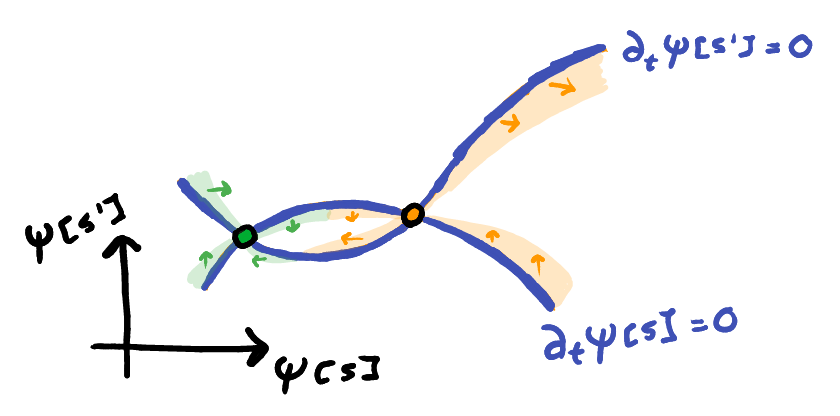
\includegraphics[scale=0.35]{figures/nullclines}
\caption{Schematic of two nullclines with their orthogonal local\\ field flows intersecting
at \textcolor{Green}{stable} and \textcolor{orange}{unstable} fixed points $\psi^*$}
\label{fig:nullclines}
\end{figure}
Nullclines determine local direction of evolution of the system. On a given
nullcline $\partial_t\psi[s]=0$ the flow of the field must be orthogonal to
the direction of $\psi[s]$. At intersections between two nullclines, the flow
must be orthogonal to the plane defined by two axes. At the interactions between
all nullcline we may find the fixed points $\psi^*$ as shown in Figure \ref{fig:nullclines}.

Classification of fixed points $\psi^*$ is done by linearising the equation of motion
\eqref{eq:reaction} with respect to field perturbation $\varepsilon(t)$ in their vicinity
and determining the eigenvalues of the resultant $S\times S$ Jacobian $\mathbf{J}(\psi)$
evaluated at each fixed point $\psi^*$.
\begin{align}
	\varepsilon(t) \sim
	\mathbb{e}^{\mathbf{J}(\psi)|_{\psi=\psi^*}t}\qquad\qquad\qquad\qquad\qquad\qquad
	\\
	\quad\text{where}\quad
	\mathrm{J}[i,j]=
	\sum_{r=1}^R
	\sigma[r]
\bigg(H(\psi[i])-H(\psi[i]-g[i,r])\bigg)
	\Gamma[j,r]
		\prod_{s=1}^S{\psi[s] \choose g[s,r]}
	\\
	H(x)=\int_0^1\frac{1-t^x}{1-t}\mathrm{d}t\quad
	\text{are generalised Harmonic Numbers}\qquad
	\label{eq:linearstability}
\end{align}
For reactions involving one or two distinguishable particles as
in \eqref{eq:simplifiedpropensity} the nullclines become hyperplanes and the Jacobian
simplifies. We can see that both the reaction topology given by stoichiometric
coefficients $\Gamma[i,j]$ and the reaction rates $\sigma[r]$ contribute to
rotating and shifting the hyperplanes and determining the location and stability
of their intersections.
\begin{align}
	\mathrm{J}[i,j]=
	\sum_{r=1}^R
		\sigma[r]|\Gamma[i,r]|\Gamma[j,r]
		\prod_{\,s\neq i}
		\psi[s]^{g[i,r]}
		\qquad g[i,r]\in\{0,1\} \quad\forall i,r
	\label{eq:simplifiedjacobian}
\end{align}
The sign of eigenvalues $\lambda$ of Jacobian $\mathbf{J}$ determine whether a fixed point
is stable $\lambda<0$ or unstable $\lambda>0$. As an illustrative example we can characterise
fixed points given an arbitrary two dimensional Jacobian. Figure \ref{fig:stability} reveals
the regions of stability and phase space flows.
\begin{figure}[H]
\centering{}
\captionsetup{justification=centering}
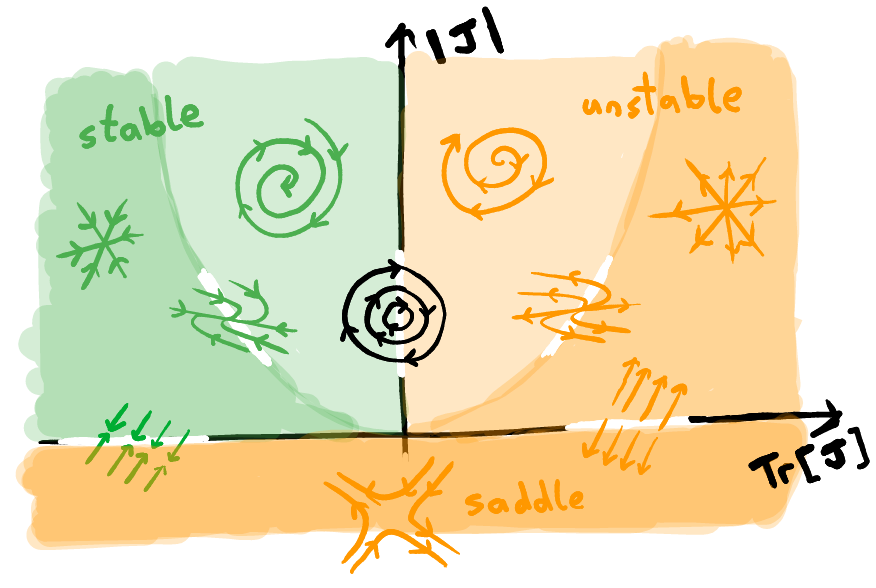
\includegraphics[scale=0.35]{figures/stability}
\caption{Classification of \textcolor{Green}{stable} and \textcolor{orange}{unstable}
fixed points for a general \\two dimensional Jacobian in terms of trace $\mathrm{Tr}[\mathbf{J}]$ and
determinant $|\mathbf{J}|$}
\label{fig:stability}
\end{figure}
Varying the continuos parameters $\sigma[r]$ moves the nullclines and may result in
the creation or annihilation of fixed points of different classes. While an individual
fixed point may change location and local phase space flow, it cannot change class
without involving another fixed point.

These are called bifurcations and also fall into various categories.
Figure \ref{fig:bifurcations} illustrates some of the possible one parameter
supercritical bifurcations; subcritical cases are obtained by permuting
stabilities of fixed points. Note the hysteresis loop in the saddle-node
bifurcation.
\begin{figure}[H]
\centering{}
\captionsetup{justification=centering}
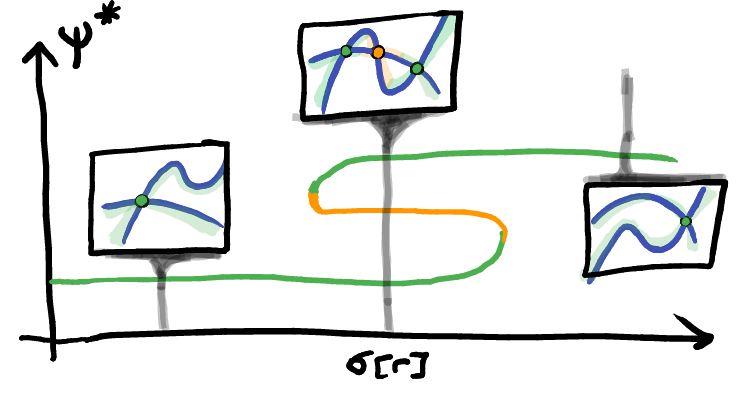
\includegraphics[scale=0.35]{figures/saddlenode}
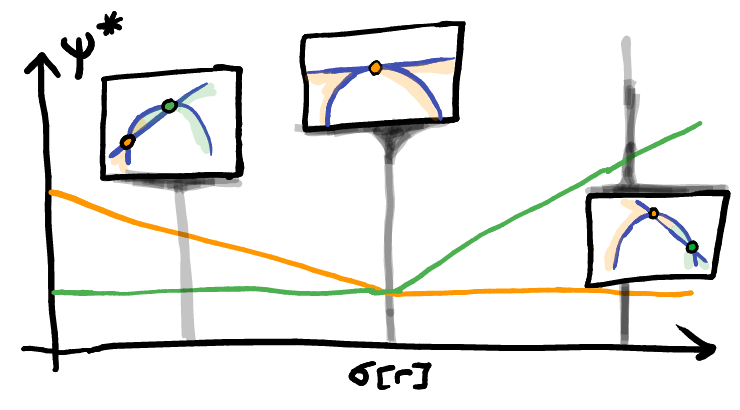
\includegraphics[scale=0.35]{figures/transcritical}
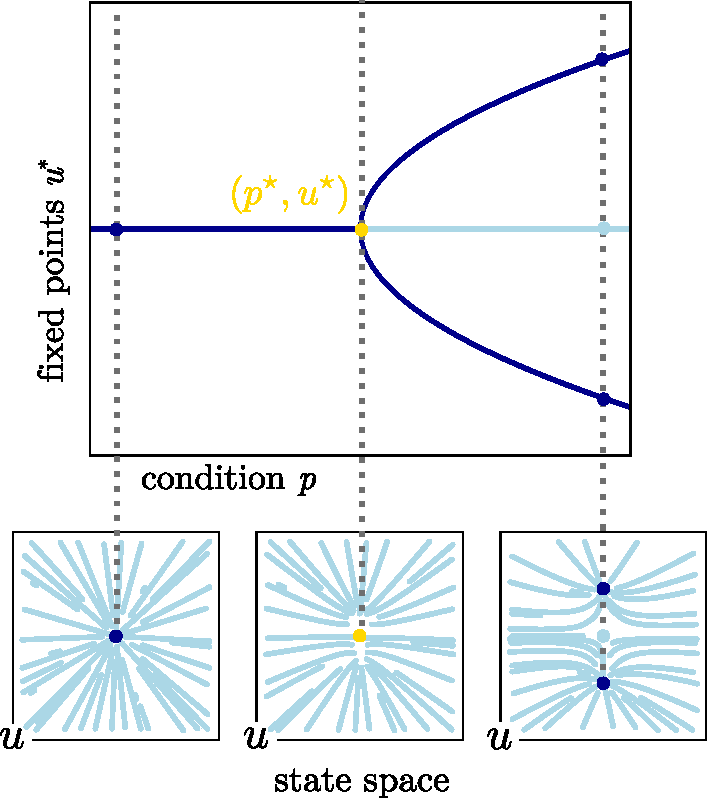
\includegraphics[scale=0.35]{figures/pitchfork}
\caption{Saddle-node, Transcritical and Pitchfork bifurcation diagram showing
\textcolor{Green}{stable} and \\\textcolor{orange}{unstable} fixed points $\psi^*$
as a function of parameter $\sigma[r]$. Insets show nullcline intersections.}
\label{fig:bifurcations}
\end{figure}
Another category of bifurcations involves limit cycles, which emerge from fixed
points where the linearised Jacobian eigenvalues have no real part. Limit cycles
have circulating field flow as shown in Figure \ref{fig:stability} along the
$\mathrm{Tr}[\mathbf{J}]=0$, $|\mathbf{J}|>0$ axis.

Note how oscillations emerge at small amplitudes in the Hopf bifurcation,
whereas the large amplitude oscillations may instantly emerge in an infinite-period
or cyclic-fold bifurcation. In Figure \ref{fig:limitcycles} the shaded regions
represent the peaks and troughs of the oscillations.
\begin{figure}[H]
\centering{}
\captionsetup{justification=centering}
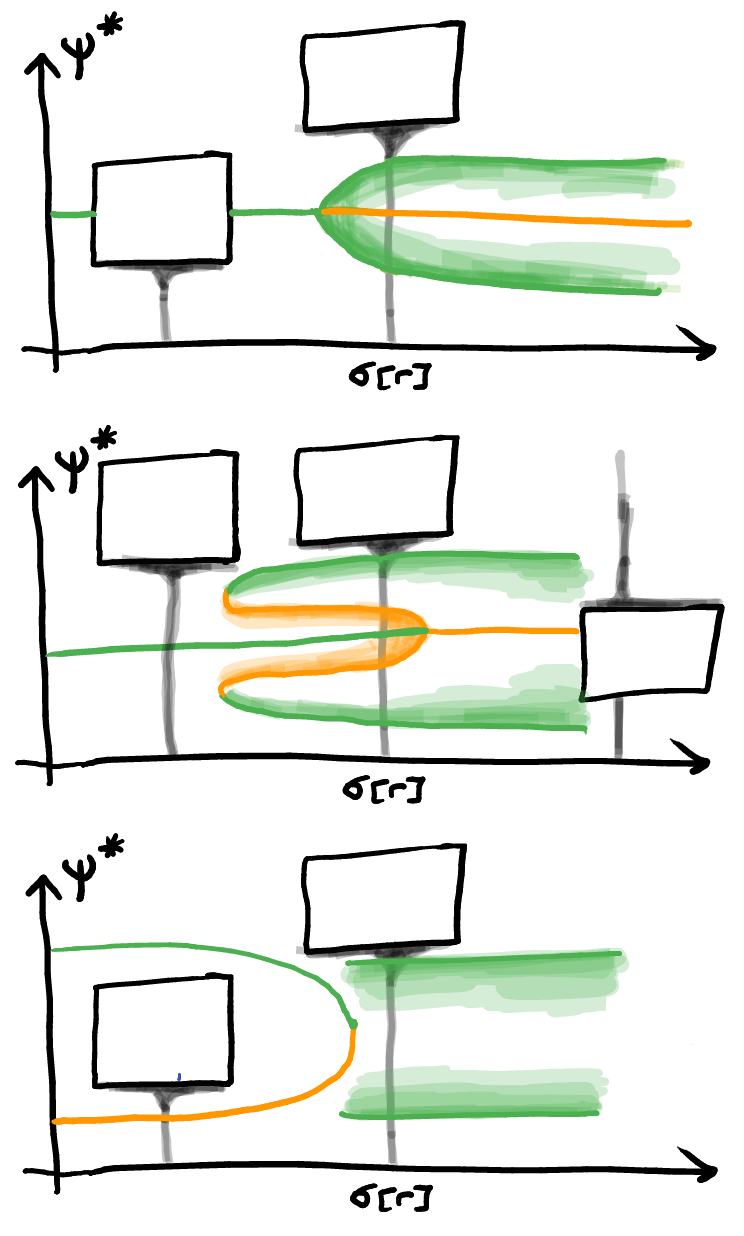
\includegraphics[scale=0.35]{figures/limitcycles}
\caption{Hopf, Cyclic-fold and Infinite-Period bifurcation diagram showing
\textcolor{Green}{stable} and \textcolor{orange}{unstable}\\ fixed points
and limit cycles as a function of parameter $\sigma[r]$.
Insets show nullclines [tbc]}
\label{fig:limitcycles}
\end{figure}
\subsection{Attractor Geometry and Universality}
In this section we would explore the geometrisation of phase space, lyapunov
exponents and universality. Perhaps a discussion on phase transitions and
the relation to Landau-Ginzberg approaches is required.
Maybe also periodic orbit theory? Depends how useful it is.
\subsection{Reaction-Diffusion}
Here we first introduce diffusion macroscopically by simply adding the laplacian
to mean field equation $\eqref{eq:reaction}$. We introduce the turning bifurcation and
show how linear stability analysis is insufficient to capture pattern formation
and rich inhomogeneous steady states. A promising approach may be geometrisation
of the moving local equilibria \cite{Halatek2018}.

\section{Phenotype Inference with Machine Learning}
\begin{itemize}
    \item Preface on SciML community and gray-box modelling
\end{itemize}

\subsection{Classification and Regression}
\begin{itemize}
    \item Logistic regression
    \item Nearest neighbour methods
    \item Mixture Models
\end{itemize}

\subsection{Dimensionality Reduction Methods}
\begin{itemize}
    \item UMAP and Tsne
    \item Sloppy parameters and identify-ability
\end{itemize}

\subsection{Clustering Methods}
